\chapter{PID controller}

My first sub-task of BTP was to train a drone in simulation to go from point A to point B without much deviations, jerks and oscillations.
It can be achieve in two ways, one by pid controller and other by training a drone by reinforcement learning. 
Its important to understand PID controller approach first, later will discuss the other approach.
\section{Introduction}

PID stands for Proportional, Integral, Derivative, it’s part of a flight controller software that reads the data from sensors and calculates how fast the motors should spin in order to retain the desired rotation speed of the aircraft.
\\
The goal of the PID controller is to correct the “error“, the difference between a measured value (gyro sensor measurement), and a desired set-point (the desired rotation speed). The “error” can be minimized by adjusting the control inputs in every loop, which is the speed of the motors.
\\
There are 3 values in a PID controller, they are the P term, I term, and D term:
\\
"P" looks at present error –  the further it is from the set-point, the harder it pushes
\\"D" is a prediction of future errors – it looks at how fast you are approaching a set-point and counteracts P when it is getting close to minimize overshoot
\\"I" is the accumulation of past errors, it looks at forces that happen over time; for example if a quad constantly drifts away from a set-point due to wind, it will spool up motors to counteract it
\\
\begin{figure}
    \centering
    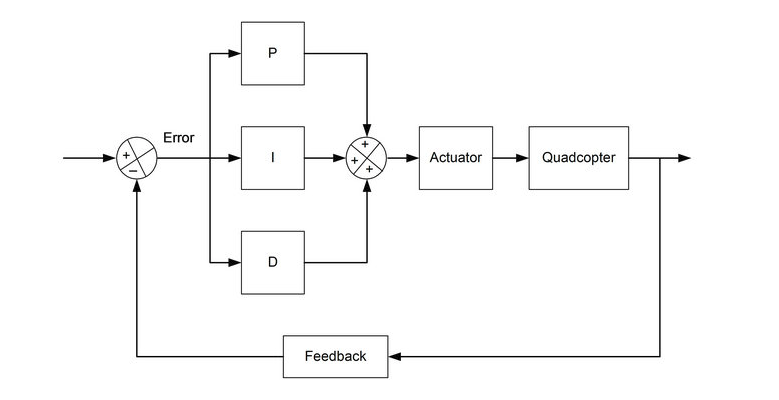
\includegraphics[width=\textwidth]{pid.png}
    \caption{PID Controller Diagram}
\end{figure}
\section{Implementation}
Here we will implement the position hold algorithm for drone using ROS in vrep software.
\subsection{ROS}
Robot Operating System(ROS) is a meta-operating system for a robot. It provides services that one would expect from an operating system, including hardware abstraction, device drivers, libraries, visualizers, low-level device control, implementation of commonly-used functionality, message-passing between processes, and package management. It also provides tools and libraries for obtaining, building, writing, and running code across multiple computers. It is named as a meta-operating system because it is something between an operating system and middleware. It provides not only standard operating system services (like hardware abstraction) but also high-level functionalities like asynchronous and synchronous calls, a centralized database, a robot configuration system, etc. ROS can be interpreted also as a software framework for robot software development, providing the operating system.ROS is based on a Unix-like philosophy of building many small tools that are designed to work together. ROS grows out of a collaboration between industry and academia and is a novel blend of professional software development practices and the latest research results.

\subsection{Pluto drone}
Drone used for this experiment is pluto drone, this is light weight drone.
\begin{figure}
    \centering
    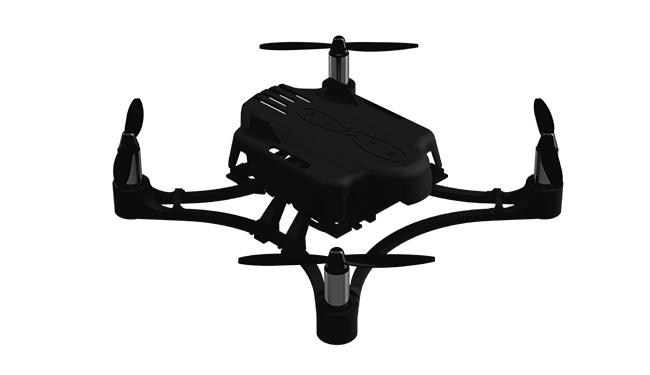
\includegraphics[width=0.5\textwidth]{images/pluto.png}
    \caption{Pluto drone}
\end{figure}

\subsection{V-REP}
V-REP is simulation software which can be used with ROS to simulated various robots.
\\
\newline \begin{figure}
    \centering
    % \caption{V-Rep simulation of pluto drone}
    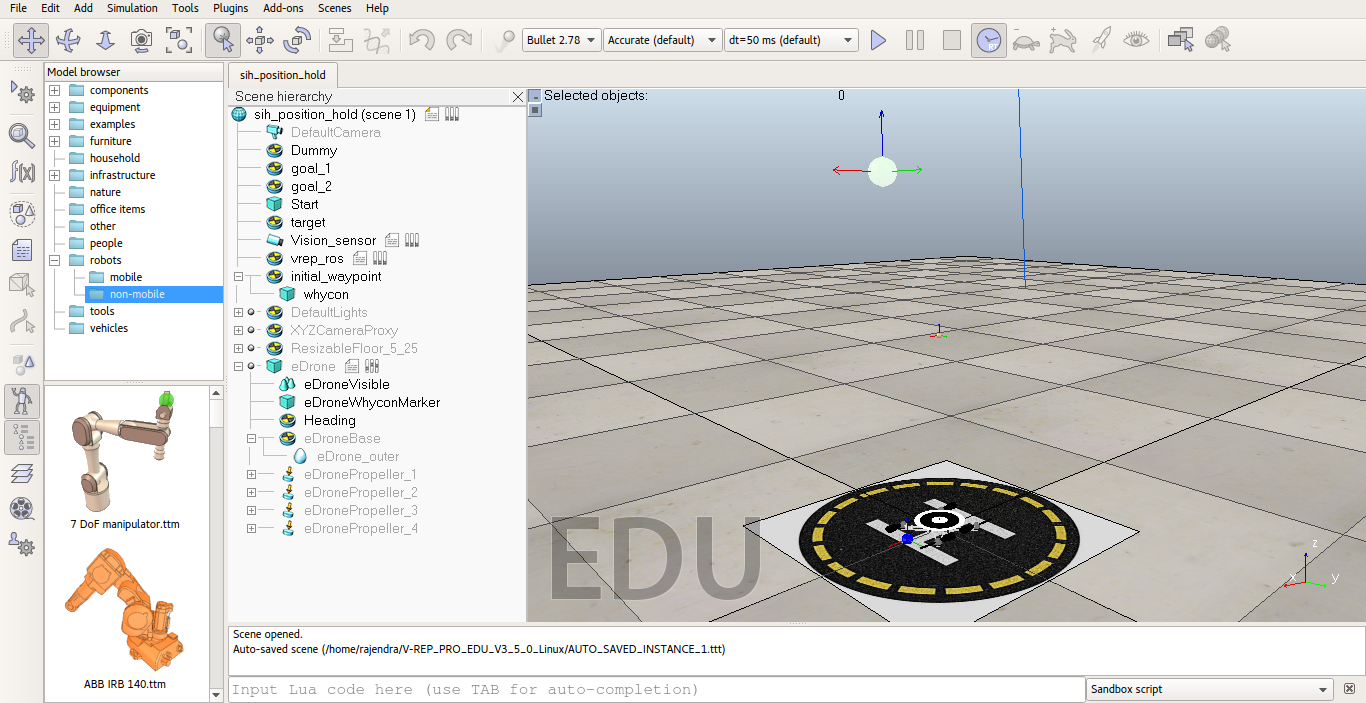
\includegraphics[width=\textwidth]{images/vrep.png}
    \\
    \caption{V-Rep simulation of pluto drone}
\end{figure}
\\
\subsection{Algorithm}
\\
Lets write the \textbf{positionHoldWhycon.py} roscode as below. It uses the position of drone we get by detecting the whycon marker on the drone and publish the drone command to hold to the given position.
% \documentclass{article}

 
% \begin{document}
\begin{minted}{python}
#!/usr/bin/env python

'''

This python file runs a ROS-node of name drone_control which holds the position of e-Drone on the given dummy.
This node publishes and subsribes the following topics:

		PUBLICATIONS			SUBSCRIPTIONS
		/drone_command			/whycon/poses
		/alt_error				/pid_tuning_altitude
		/pitch_error			/pid_tuning_pitch
		/roll_error				/pid_tuning_roll
		/yaw_error				/pid_tuning_yaw
								/drone_yaw
'''
# ========== Importing the required libraries =============#
from plutodrone.msg import *
from geometry_msgs.msg import PoseArray
from std_msgs.msg import Int16
from std_msgs.msg import Int64
from std_msgs.msg import Float64
from pid_tune.msg import PidTune
import rospy
import time

class Edrone():
	"""docstring for Edrone"""
	def __init__(self):
		rospy.init_node('drone_control')	# initializing ros node with name drone_control
		# This corresponds to your current position of drone. This value must be updated each time in your whycon callback
		# [x,y,z,yaw_value]
		self.drone_position = [0.0,0.0,0.0,0.0]	
		# [x_setpoint, y_setpoint, z_setpoint, yaw_value_setpoint]
		self.setpoint = [-8.39, 4.98, 27.92, 0.0] # whycon marker at the position of the dummy given in the scene. Make the whycon marker associated with position_to_hold dummy renderable and make changes accordingly
		#Declaring a cmd of message type PlutoMsg and initializing values
		self.cmd = PlutoMsg()
		self.cmd.rcRoll = 1500
		self.cmd.rcPitch = 1500
		self.cmd.rcYaw = 1500
		self.cmd.rcThrottle = 1500
		self.cmd.rcAUX1 = 1500
		self.cmd.rcAUX2 = 1500
		self.cmd.rcAUX3 = 1500
		self.cmd.rcAUX4 = 1500
		# self.cmd.plutoIndex = 0
		#initial setting of Kp, Kd and ki for [pitch, roll, throttle, yaw]. eg: self.Kp[2] corresponds to Kp value in throttle axis
		#after tuning and computing corresponding PID parameters, change the parameters
		self.Kp = [5.13, 12, 23.1, 9]
		self.Ki = [0.8 , 0, 0, 0.1496]
		self.Kd = [13.365, 58.5, 342.9, 112.83]
		#------Add other required variables for pid here-----------
		self.prev_values = [0,0,0,0]
		self.max_values = [1700,1700,1800,1800]
		self.min_values = [1300,1300,1200,1200]
		self.sum_of_error = [0.0, 0.0, 0.0, 0.0]
		self.output = [0.0, 0.0, 0.0, 0.0]
		self.iterm = [0,0,0,0]
		#-----------------------------------------------------------
		# This is the sample time in which run pid.
		self.sample_time = 0.10 # in seconds
		self.error_pub = [0.0, 0.0, 0.0, 0.0]
		self.zero_line = 0
		# Publishing /drone_command, /alt_error, /pitch_error, /roll_error, /yaw_error
		self.command_pub = rospy.Publisher('/drone_command', PlutoMsg, queue_size=1)
		#---------------Add other ROS Publishers here--------------
		self.error_pub[0] = rospy.Publisher('/pitch_error', Float64, queue_size=1)
		self.error_pub[1] = rospy.Publisher('/roll_error', Float64, queue_size=1)
		self.error_pub[2] = rospy.Publisher('/alt_error', Float64, queue_size=1)
		self.error_pub[3] = rospy.Publisher('/yaw_error', Float64, queue_size=1)
		self.zero_line = rospy.Publisher('/zero_line', Float64, queue_size=1)
		#-----------------------------------------------------------
		# Subscribing to /whycon/poses, /drone_yaw, /pid_tuning_altitude, /pid_tuning_pitch, pid_tuning_roll
		rospy.Subscriber('whycon/poses', PoseArray, self.whycon_callback)
		rospy.Subscriber('/pid_tuning_altitude',PidTune,self.altitude_set_pid)
		#----------Add other ROS Subscribers here-------------
		rospy.Subscriber('/pid_tuning_pitch',PidTune,self.pitch_set_pid)
		rospy.Subscriber('/pid_tuning_roll',PidTune,self.roll_set_pid)
		rospy.Subscriber('/pid_tuning_yaw',PidTune,self.yaw_set_pid)
		rospy.Subscriber('/drone_yaw',Float64, self.droneYaw)
		#-----------------------------------------------------------
		self.arm() #ARMING THE DRONE
	
	# Disarming condition of the drone
	def disarm(self):
		self.cmd.rcAUX4 = 1100
		self.command_pub.publish(self.cmd)
		rospy.sleep(1)

	# Arming condition of the drone : Best practise is to disarm and then arm the drone.
	def arm(self):
		self.disarm()
		self.cmd.rcRoll = 1500
		self.cmd.rcYaw = 1500
		self.cmd.rcPitch = 1500
		self.cmd.rcThrottle = 1000
		self.cmd.rcAUX4 = 1500
		self.command_pub.publish(self.cmd)	# Publishing /drone_command
		rospy.sleep(1)

	# Whycon callback function
	# The function gets executed each time when /whycon node publishes /whycon/poses 
	def whycon_callback(self,msg):
		self.drone_position[0] = msg.poses[0].position.x
		#-----Set the remaining co-ordinates of the drone from msg--
		self.drone_position[1] = msg.poses[0].position.y
		self.drone_position[2] = msg.poses[0].position.z
		#-----------------------------------------------------------

	# Callback function for /pid_tuning_altitude
	# This function gets executed each time when /tune_pid publishes /pid_tuning_altitude
	def altitude_set_pid(self,alt):
		self.Kp[2] = alt.Kp * 0.06 # This is just for an example. You can change the fraction value accordingly
		self.Ki[2] = alt.Ki * 0.008
		self.Kd[2] = alt.Kd * 0.3
	
	#----Define callback function like altitide_set_pid to tune pitch, roll and yaw as well-------
	def pitch_set_pid(self, pit):
		self.Kp[0] = pit.Kp * 0.006
		self.Ki[0] = pit.Ki * 0.008
		self.Kd[0] = pit.Kd * 0.003

	def roll_set_pid(self, rl):
		self.Kp[1] = rl.Kp * 0.06
		self.Ki[1] = rl.Ki * 0.008
		self.Kd[1] = rl.Kd * 0.0375

	def yaw_set_pid(self, yw):
		self.Kp[3] = yw.Kp * 0.006 
		self.Ki[3] = yw.Ki * 0.0008
		self.Kd[3] = yw.Kd * 0.03

	def droneYaw(self, yw):
		self.drone_position[3] = yw.data
	#-----------------------------------------------------------
	def setRange(self):
		for i in range (0, 4):
			if self.output[i] > self.max_values[i] :
				self.output[i] = self.max_values[i]
			elif self.output[i] < self.min_values[i] :
				self.output[i] = self.min_values[i]

		if self.cmd.rcPitch > self.max_values[0]:
		 	self.cmd.rcPitch = self.max_values[0]
		elif self.cmd.rcPitch < self.min_values[0]:
		 	self.cmd.rcPitch = self.min_values[0]

		if self.cmd.rcRoll > self.max_values[1]:
		 	self.cmd.rcRoll = self.max_values[1]
		elif self.cmd.rcRoll < self.min_values[1]:
		 	self.cmd.rcRoll = self.min_values[1]

		if self.cmd.rcThrottle > self.max_values[2]:
		 	self.cmd.rcThrottle = self.max_values[2]
		elif self.cmd.rcThrottle < self.min_values[2]:
		 	self.cmd.rcThrottle = self.min_values[2]

		if self.cmd.rcYaw > self.max_values[3]:
		 	self.cmd.rcYaw = self.max_values[3]
		elif self.cmd.rcYaw < self.min_values[3]:
		 	self.cmd.rcYaw = self.min_values[3]

	def pid(self):
	#------------- PID algorithm here-------------------------
	# Steps:
	# 	1. Compute error in each axis. eg: error[0] = self.drone_position[0] - self.setpoint[0] ,where error[0] corresponds to error in x...
	#	2. Compute the error (for proportional), change in error (for derivative) and sum of errors (for integral) in each axis.
	#	3. Calculate the pid output required for each axis. For eg: calcuate self.out_roll, self.out_pitch, etc.
	#	4. Reduce or add this computed output value on the avg value ie 1500.EXPERIMENT AND FIND THE CORRECT SIGN
	#	5. Don't run the pid continously. Run the pid only at the a sample time. self.sampletime defined above is for this purpose.
	#	6. Limit the output value and the final command value between the maximum(1800) and minimum(1200)range before publishing.
	#	7. Update previous errors.eg: self.prev_error[1] = error[1] where index 1 corresponds to that of pitch
	#	8. Add error_sum
	
		error = [0.0, 0.0, 0.0, 0.0]
		change_in_error = [0.0, 0.0, 0.0, 0.0]
		for i in range (0, 4):
			error[i] = self.setpoint[i] - self.drone_position[i]
			self.error_pub[i].publish(error[i])
			change_in_error[i] = error[i] - self.prev_values[i]
			self.sum_of_error[i] = self.sum_of_error[i] + error[i]
			self.iterm[i] = self.iterm[i] + (error[i] * self.Ki[i])
			self.output[i] = (self.Kp[i] * error[i]) + self.iterm[i] + (self.Kd[i] * change_in_error[i])
			self.prev_values[i] = error[i]
			
		self.cmd.rcPitch = 1500 - self.output[0]
		self.cmd.rcRoll = 1500 - self.output[1]
		self.cmd.rcThrottle = 1500 - self.output[2]
		self.cmd.rcYaw = 1500 + self.output[3]
		
		self.setRange()
		self.command_pub.publish(self.cmd)
		self.zero_line.publish(0.0)
		rospy.sleep(self.sample_time)
	#--------------------------------------------------------------#
if __name__ == '__main__':
	e_drone = Edrone()
	while not rospy.is_shutdown():
		e_drone.pid()
\end{minted}

\section{Conclusion}

I was able to hold the drone to given position but it required a lot and very precise pid tuning to get there.
Hence, PID control based algorithm is easy and intuitive to understand but hard to improve and tune.
% \end{document}